\documentclass{article}
\usepackage{polski}
\usepackage[utf8]{inputenc}
\usepackage{amsmath}
\usepackage{amsthm}
\usepackage{amssymb}
\usepackage{graphicx} 
\usepackage{mathtools}
\title{Fizyka Statystyczna i Termodynamika \\ Opracowanie zagadnień do egzaminu}
\author{Katarzyna Kosek \\ Patryk Bojarski}

\begin{document}
	\maketitle
	\newpage
	\pagenumbering{arabic}
	\section{Wykład 1}
		\paragraph{Literatura:}
			\begin{itemize}
				\item \textit{Termodynamika dla chemików i fizyków} R. Hołyst
				\item \textit{Termodynamika fenomenologiczna} J. Werle
				\item \textit{Fizyka statystyczna} A. Zagórski
				\item \textit{Wykłady z mechaniki statystycznej} R. Feynmann
			\end{itemize}
		\paragraph{Wielkości ekstensywne:} są proporcjonalne do wielkości układu: $S(u) = S(u_1) + S(u_2)$. Przykłady: masa, energia, pęd, moment pędu, liczba cząstek
		\paragraph{Wielkości intensywne:} są niezależne od wielkości układu, przykłady: prędkość, gęstość, przyśpieszenie, potencjał chemiczny, temperatura
		\paragraph{Zmienne: }
			\begin{itemize}
				\item układu
				\item procesu (np. ciepło, praca)
			\end{itemize}
		\paragraph{Proces termodynamiczny:} quasi-statyczny układ przechodzi przez ciąg stanów równowagi
		\paragraph{Proces odwracalny:} taki proces, że jeżeli odwrócimy zmianę warunków zewnętrznych to układ wróci do poprzedniego stanu.
		\paragraph{Układ termodynamiczny:}
			\begin{itemize}
				\item izolowany: $\Delta E = 0, \Delta N = 0$
				\item zamknięty: $\Delta N = 0$
				\item otwarty
			\end{itemize}
		\paragraph{Zasady termodynamiki}
			\subparagraph{0} Dla każdego układu termodynamicznego w stanie równowagi istnieje intensywna funkcja stanu $\theta$ zwana \textbf{temperaturą}, taka że jeżeli jest:
				\begin{itemize}
					\item w równowadze z II
					\item w równowadze z III
				\end{itemize}
			to I jest w równowadze z III - przechodniość stanów nierównowagowych termodynamicznych: $\theta_2 > \theta_1$.
			\subparagraph{1} Dla każdego układu termodynamicznego istnieje ekstensywna wielkość zwana \textbf{energią wewnętrzną U} będącą sumą wszystkich typów energii w układzie. Ponadto w układach izolowanych $U = const$.
			$$\delta E = \sum_i X_id \tilde{x}_i$$
			Gdzie $X_i$ to zmienna intensywna a $ \tilde{x}_i$ to zmienna ekstensywna. \\
			$U$ można zmienić poprzez:
				\begin{itemize}
					\item dostarczenie (odebranie) ciepła dQ xt	
					\item $dW > 0$, $dW < 0$ - praca wykonywana przez układ
					\item dZ  - przepływ materii
				\end{itemize}
	\section{Wykład 2}
			\subparagraph{2} Istnieje intensywna zmienna zwana temperaturą bezwzględną $T > 0$, oraz ekstensywna zmienna S zwana \textbf{entropią} $TdS = dQ$. Entropia układu izolowanego nigdy nie maleje i w stanie równowagi osiąga maksimum zależne od warunków brzegowych
			\begin{figure}[ht]
				\label{fig:fig1}
				\centering
				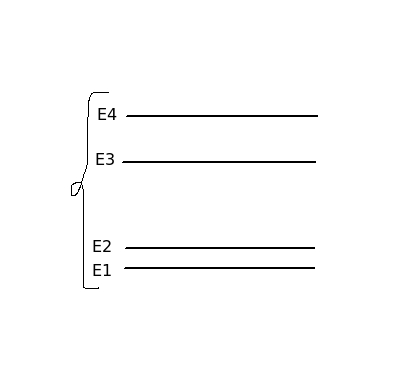
\includegraphics[scale=0.4]{poziomyenergetyczne.jpeg}
				\caption{Poziomy energetyczne}
			\end{figure}
			$$p ~ exp[-\beta\varepsilon_k]$$	
			To jest prawdopodobieństwo a 
			$$\beta = \frac{1}{k_BT}$$
			to czynnik Boltzmanowski.
			$$dS = dS_e + dS_i$$
			To znaczy entropia jest równa $dS_e = \frac{dQ}{T}$ i $dS_i$ - entropii tworzenia w układzie (i - internal, e - external).
			\begin{figure}[ht]
				\label{fig:fig1}
				\centering
				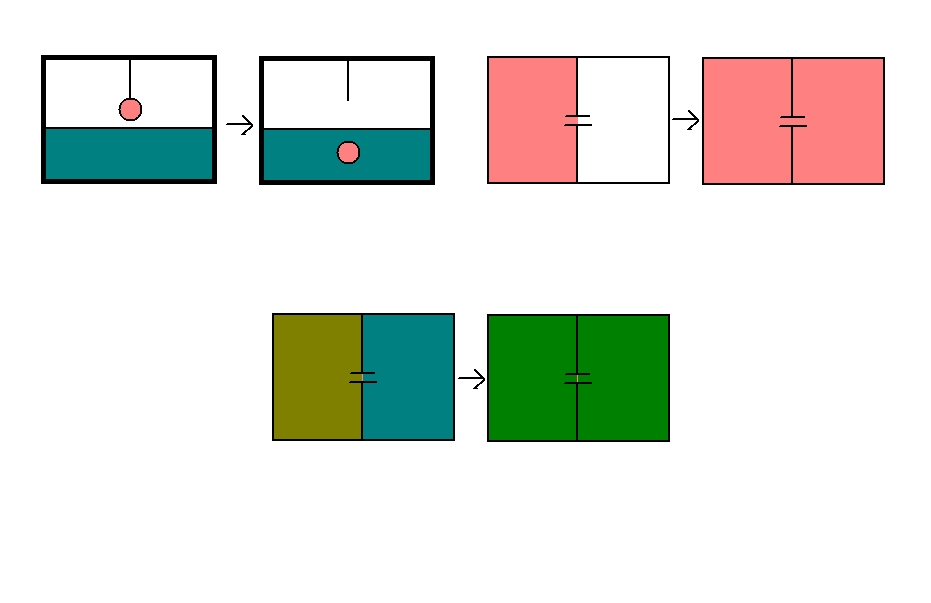
\includegraphics[scale=0.6]{entropiamieszania.jpeg}
				\caption{Entropia mieszania}
			\end{figure}		
			Dla powyższych procesów nieodwracalnych $dS_i > 0$. \\
			$dS_i = 0 $
			\begin{figure}[ht]
			\label{fig:fig1}
			\centering
			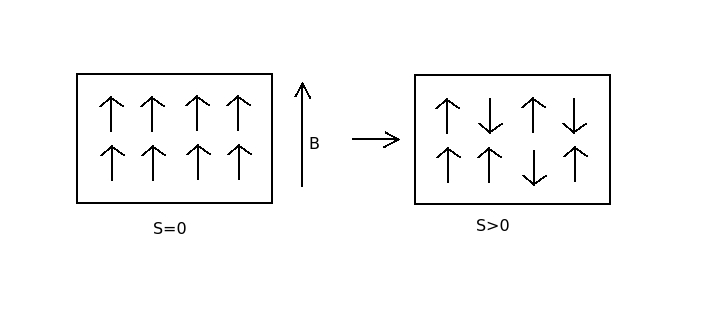
\includegraphics[scale=0.6]{chlodzeniemagnetyczne.jpeg}
			\caption{Chłodzenie magnetyczne}
			\end{figure}

			\begin{figure}[ht]
				\label{fig:fig1}
				\centering
				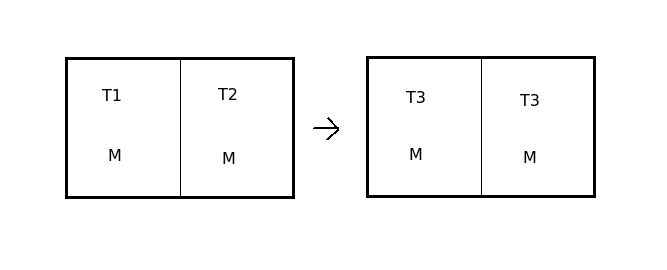
\includegraphics[scale=0.6]{temperatury.jpeg}
				\caption{Entropia w układzie bez mieszania materii}
			\end{figure}
			
			Entropia dla dwóch układów wymieniających ciepło ale nie temperaturę:
			$$dS_1 = \frac{dQ_1}{T_1}$$		
			$$dS_2 = \frac{dQ_2}{T_2}$$
			$$0 < dQ_1 = -dQ_2$$
			$$dS = dS_1 + dS_2 = \frac{dQ_1}{T_1} + \frac{dQ_2}{T_2} = dQ_2(\frac{1}{T_1} + \frac{1}{T_2})$$	
			
			\begin{figure}[ht]
				\label{fig:fig1}
				\centering
				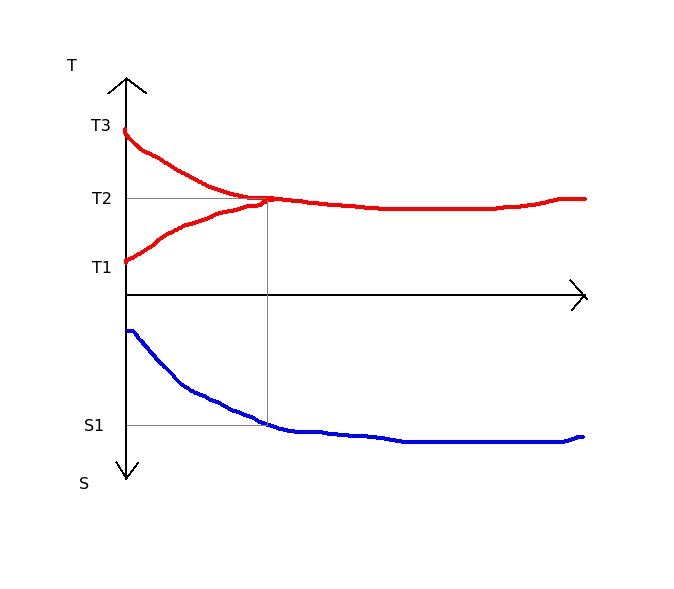
\includegraphics[scale=0.6]{nieodwracalneprocesy.jpeg}
				\caption{Dojście do stanu równowagi}
			\end{figure}
			
			Wiele nieodwracalnych procesów odpowiada za dojście do stanu równowagi.
			$$dS = dS_e + dS_i$$
			$$S = k_b ln(\Omega)$$
			$\Omega$ - liczba mikrostanów
		\paragraph{Transformacja Legendre'a}
			$$g(f'(x)) = f(f'(x)) - xf'(x)$$
			$$U = U(S, V, N)$$
			$$dU = TdS - pdV$$
			$$T = (\frac{\partial U}{\partial S})_{V,N}$$
			$$p = (\frac{\partial U}{\partial V})_{S,N}$$
			$$\frac{\partial^2U}{\partial U \partial S} = (\frac{\partial T}{\partial V})_{S,N}$$
			$$\frac{\partial ^ 2 U}{\partial S \partial V} = (\frac{\partial p}{\partial S})_{V.N}$$
			$$F(T,V,N) = U(S(T), V, N) - S(\frac{\partial U}{\partial S})_{V,N}$$
			\textbf{F} - energia swobodna Helmholtza
			$$dF = d(U - S\frac{\partial U}{\partial S}) = d(U - ST) = TdS - pdV + \mu dN - (TdS + SdT) = -SdT - pdV + \mu dN$$
			$$(\frac{dF}{dT})_{V,N} = -S$$
			Pochodna jest przy stałych V i N, bo w drugim członie równania na dF jest tak samo.
			$$H(S,P,N) = U(S, V(p), N) - U(\frac{\partial U}{\partial V})_{S,N} = U(S, V(p), N) + pV$$
			\textbf{H} - entalpia
			$$dH = d(U + pV) = TdS - pdV + \mu dN + pdV + Vdp = TdS + Vdp + \mu dN$$
			$$(\frac{\partial H}{\partial S})_{p,N} = T$$
			$$(\frac{\partial H}{\partial p})_{S,N} = V$$
			$$(\frac{\partial T}{\partial p})_{S,N} = (\frac{\partial V}{\partial S})_{p,N}$$
			To wyżej to relacja Maxwella.
			$$G(T, P, N) = U - S(\frac{\partial U}{\partial S})_{V,N} - V(\frac{\partial U}{\partial V})_{S,N} = U - TS + pV$$
			$$G = H - TS \Rightarrow dG = -SdT + Vdp ++ \mu dN$$
			$$G = \mu N$$
			To wyżej - \textbf{prawo Gibbsa - Duhlema}\\
			\textbf{G} - entalpia swobodna.
	\section{Wykład 3}
		$$U_2(S,V,N) = \lambda U(S,V,N) = U(\lambda S, \lambda V, \lambda N)$$
		$$\frac{\partial U}{\partial \lambda} \Big |_{\lambda = 1} = TS - pV + \mu N = U(S,V,N)$$
		$$U = TS + pV = \mu N \Rightarrow G = \mu N$$
		$$dG = -SdT + Vdp + \mu dN$$
		\paragraph{Zasada pracy maksymalnej} Układ wykonuje pracę kosztem swojego odpowiedniego potencjału termodynamicznego. Praca jest maksymalna dla procesów odwracalnych (tutaj N=const, dN = 0, układ zamknięty).
		$$dY = dQ + dW$$
		I zasada termodynamiki
		$$dS = dS^e + dS^i = \frac{dQ}{T} + dS^i \geqslant 0$$			
		Równanie ciągłości entropii
		$$dS \geqslant \frac{dQ}{T}$$
		Powyższa równość zachodzi dla $dS^i = 0$, czyli dla procesów odwracalnych.
		$$TdS \geqslant dQ$$
		Wykorzystując powyższą nierówność i I zasadę termodynamiki:
		$$dU \leqslant dW + TdS$$
		\textbf{dW} - praca wykonywana nad układem.
		$$dU \leqslant d \widetilde{W} + TdS$$
		$d\widetilde{W} = -dW$ - praca wykonywana przez układ
		$$d\widetilde{W} \leqslant TdS - dU$$
		gdy $dS = 0$, to $d\widetilde{W} \leqslant -dU$
		\subparagraph{Wniosek:} przy \textbf{S=const} praca wykonywana jest kosztem \textbf{energii wewnętrznej}
		\paragraph{}
		$$F = U - TS$$
		Energia swobodna Helmholtza.
		$$dF = dU - TdS - SdT = dQ + dW - TdS - SdT$$
		Wykorzystując nierówność $dS \geqslant \frac{dQ}{T}$ i $d\widetilde{W} = -dW$
		$$dF \leqslant TdS - d\widetilde{W} - TdS - SdT$$
		$$dF \leqslant -d\widetilde{W} - SdT$$
		$$d \widetilde{W} \leqslant -dF -SdT$$
		gdy $dT = 0$, to $d\widetilde{W} \leqslant -dF$
		\subparagraph{Wniosek:} przy \textbf{T=const} (proces izotermiczny) praca wykonywana jest kosztem \textbf{energii swobodnej Helmholtza}.
		\paragraph{}
		$$H = U + pV$$
		$$dH = dU + pdV + Vdp = dQ + dW + pdV + Vdp$$
		Wykorzystując nierówność $dS \geqslant \frac{dQ}{T}$ i $d\widetilde{W} = -dW$
		$$dH \leqslant TdS - d \widetilde{W} + pdV + Vdp$$
		gdzie pdV to praca objętościowa $d\widetilde{W}_V$
		$$(d\widetilde{W} - d\widetilde{W}_V) \leqslant -dH + TdS + Vdp$$
		gdy $S = 0$ i $dp = 0$, to $(d\widetilde{W} - d\widetilde{W}_V) \leqslant -dH$
		\subparagraph{Wniosek:} przy \textbf{S=const} i \textbf{p=const} praca \textbf{nieobjętościowa} wykonywana jest kosztem \textbf{entalpii}. 
		\paragraph{}
		$$G = U - TS + pV$$
		Powyżej: entalpia swobodna.
		$$dG = dU - TdS - SdT + pdV + Vdp = dQ + dW - TdS - SdT + pdV + Vdp$$
		Wykorzystując nierówność $dS \geqslant \frac{dQ}{T}$ i $d\widetilde{W} = -dW$
		$$dG \leqslant TdS - d\widetilde{W} - SdT + pdV + Vdp$$
		gdzie $pdV$ to praca objętościowa $d\widetilde{W}_V$
		$$(d\widetilde{W} - d\widetilde{W}_V) \leqslant -dG - SdT + Vdp$$
		gdy $dT=0$ i $dp=0$, to $$(d\widetilde{W} - d\widetilde{W}_V) \leqslant - dG$$
		\paragraph{Zasada równowagi termodynamicznej} W odpowiednich warunkach narzuconych przez otoczenie, minimum przyjmuje odpowiedni potencjał termodynamiczny.
		$$U = U(S,V,N)$$
		$$dU = dQ - pdV + \mu dN$$
		Korzystając z $dS \geqslant \frac{dQ}{T}$ 
		$$dU \leqslant TdS - pdV + \mu N$$
		Przy $dS=0$ $(S=const)$, $dV = 0$ $(V=const)$, $dN=0$ $N=const$:
		$$dU \leqslant 0 \Rightarrow U = U_{min}$$
		\paragraph{}
		$$F = F(T,V,N)$$
		$$dF = dU - TdS - SdT = dQ - pdV - TdS - SdT + \mu dN$$
		Korzystając z $dS \geqslant \frac{dQ}{T}$ 
		$$dF \leqslant TdS - pdV - TdS - SdT + \mu dN = -pdV - SdT + \mu dN$$
		Przy $dV=0$ \textbf{(V=const)}, $dT=0$ \textbf{(T=const)}, $dN=0$, \textbf{(N=const)}:
		$$dF \leqslant 0 \Rightarrow F = F_{min}$$
		$$F = U - TS$$
		gdy $T = 0$ to $F_{min} = U_{min}$
		\paragraph{}
		$$H = H(S,p,N)$$
		$$dH = dU + pdV + Vdp = dQ - pdV + \mu dN + pdV + Vdp$$
		Korzystając z $dS \geqslant \frac{dQ}{T}$ 
		$$dH \leqslant TdS + Vdp + \mu dN$$
		Przy $dS=0$, \textbf{(S=const)}, $dp=0$ \textbf{(p=const)}, $dN=0$ \textbf{(N=const)}:
		$$dH \leqslant 0 \Rightarrow H=H_{min}$$
		$H = U + pV$ gdy $p=0$ to $H_{min} = U_{min}$
		\paragraph{}
		$$G = G(T,p,N)$$
		$$dG = dU - TdS - SdT + pdV + Vdp = dQ - pdV + \mu dN - TdS - SdT + pdV + Vdp$$
		Korzystając z $dS \geqslant \frac{dQ}{T}$ 
		$$dG \leqslant TdS = \mu dN - TdS - SdT + Vdp = -SdT + Vdp + \mu dN$$
		Przy $dT=0$, \textbf{(T=const)}, $dp=0$ \textbf{(p=const)}, $dN=0$ \textbf{(N=const)}:
		$$dG \leqslant 0 \Rightarrow G = G_{min}$$
		$G = U - TS + pV$, gdy $T,p = 0$ to $G_{min} = U_{min}$
		\paragraph{}
		$$dU = dW + dQ$$
		(przy N=const)
		$$dU = -pdV + dQ$$
		$$dU = dQ$$
		(przy V=const - przemiana izochoryczna)
		$$(\frac{\Delta U}{\Delta T})_V = (\frac{\Delta Q}{\Delta T}) = C_v$$
		\paragraph{}
		$$H = U + pV$$
		$$dH = dU + pdV + Vdp = dQ - pdV + pdV + Vdp = dQ + Vdp$$
		$$dH = dQ$$
		(p=const, przemiana izobaryczna)
		$$(\frac{dH}{dT})_p = C_p \Rightarrow \int_{Q_k}^{Q_p}dQ = \int_{H_p}^{H_k}dH
		\Rightarrow Q_k - Q_p = H_k - H_p$$
		Entalpia jest funkcją stanu więc $H_k$ i $H_p$ nie zależą od drogi $\Rightarrow$ $Q_k$ i $Q_p$ również nie zależą od drogi.
		
		$$C + \frac{1}{2}O_2 \longrightarrow CO$$
		$$CO + \frac{1}{2}_2 \longrightarrow CO_2$$
		$$C + O_2 \longrightarrow CO_2$$
		
		$$Q_S^{(1)} + Q_S^{(2)} = Q_S^{(3)}$$
		Powyżej: \textbf{prawo Hessa}.
	\section{Wykład 4}
		\paragraph{Prawo Kirchoffa}
		Rozpatrzmy spalanie, topnienie, wrzenie bądź sublimację:		
			\begin{figure}[ht]
				\label{fig:fig1}
				\centering
				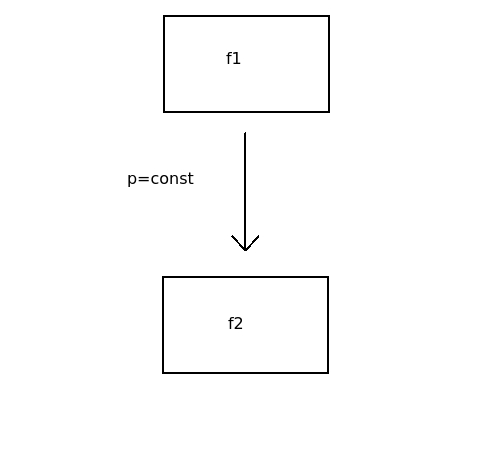
\includegraphics[scale=0.6]{prawokirchoffa.jpeg}
				\caption{Prawo Kirchoffa}
			\end{figure}
		$$Q = H_2 - H_1$$
		Powyżej: ciepło przemiany fazowej.
		$$(\frac{\partial Q}{\partial T})_p = (\frac{\partial H_2}{\partial T})_p - (\frac{\partial H_1}{\partial T})_p$$
		$(\frac{\partial H_2}{\partial T})_p$ - ciepło właściwe w fazie 1 \\
		$(\frac{\partial H_1}{\partial T})_p$ - ciepło właściwe w fazie 2 \\
		\paragraph{} Ciepło parowania wody w temperaturze $100^0 C$, pod ciśnieniem 1013hPa wynosi $Q^p = 2253 \frac{J}{g}$, ciepło właściwe pary wynosi $C_p^c = 4,187 \frac{J}{gK}$, a ciepło właściwe cieczy wynosi $C_p^c = 4,18\frac{J}{gK}$. Ile będzie wynosiło ciepło parowania w $80^0C$?
		\paragraph{Stabilność układów termodynamicznych} 
			\begin{figure}[ht]
				\label{fig:fig1}
				\centering
				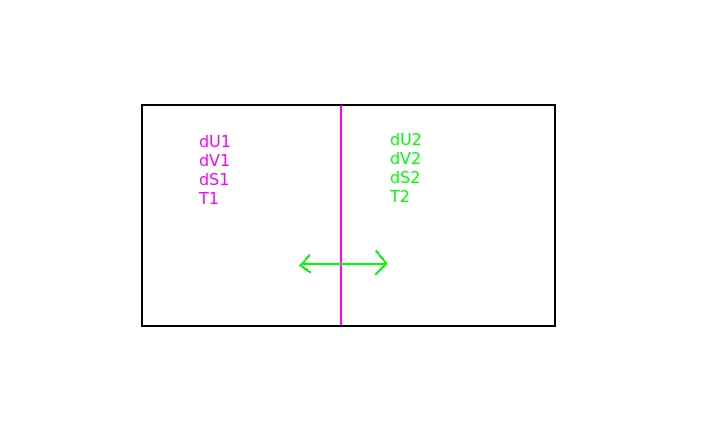
\includegraphics[scale=0.6]{stabilnoscukladow.jpeg}
				\caption{Stabilność układów termodynamicznych}
			\end{figure}
		$$dS = dS_1 + dS_2$$
		$$V = V_1 + V_2 \Rightarrow dV_1 = -dV_2$$
		$$U = U_1 + U_2 \Rightarrow dU_1 = -dU_2$$
		$$T_1dS_1 + T_2dS_2 = 0$$
		Powyższe równanie wynika z $ dQ = TdS $
		\begin{equation}
			T_1dS_1 + T_2dS_2 = 0 \Rightarrow dS_1(T_1 - T_2) = 0 \Rightarrow T_1 = T_2
		\end{equation}
		Rozwijamy dS w szereg Taylora względem zmiennych dV i dU:
		\begin{equation}
		dS = dS_1 + dS_2 = 
		(\frac{\partial S_1}{\partial U_1})dU_1 +
		\frac{1}{2}(\frac{\partial^2S_1}{\partial U_1^2})dU_1^2 +
		\frac{\partial S_1}{\partial V_1}dV_1 + 
		\frac{1}{2} (\frac{\partial^2 S_1}{\partial V_1^2})(dV_1)^2 + 
		\frac{1}{2} (\frac{\partial^2 S_1} {\partial U_1 \partial V_1})dU_1dV_1 +
		\frac{\partial S_2}{\partial U_2})dU_1 +
		\frac{1}{2}(\frac{\partial^2S_2}{\partial U_2^2})dU_2^2 +
		\frac{\partial S_2}{\partial V_2})dV_2 + 
		\frac{1}{2} (\frac{\partial^2 S_2}{\partial V_2^2})(dV_2)^2 + 
		\frac{1}{2} (\frac{\partial^2 S_2} {\partial U_2 \partial V_2})dU_2dV_2
		\end{equation}
		\begin{equation}
		dS \leqslant 0
		\end{equation}
		Przyjmujemy ża dla $ dV_1 $ i $ dV_2 $ jest równe zeru: $ V_1, V_2 = const$
		
		\begin{equation}
			dS = 
			(\frac{\partial S_1}{\partial U_1})dU_1 + 
			\frac{1}{2}(\frac{\partial^2S_1}{\partial U_1^2})dU_1^2 + 
			(\frac{\partial S_2}{\partial U_2})dU_1 +
			\frac{1}{2}(\frac{\partial^2S_2}{\partial U_2^2})dU_2^2 \leqslant 0
		\end{equation}
		
		\begin{equation}
			dS = 
			(\frac {1} {T_1})dU_1 + 
			\frac{1}{2}(\frac{\partial (\frac{1}{T})}{\partial U_1^2})dU_1^2 + 
			\frac{1}{2}(\frac{\partial (\frac{1}{T})}{\partial U_2^2})dU_2^2
		\end{equation}
		
		Tu jest jakieś równianie którego nie mogę rozczytać.\\
		Wykorzystując (1):
		\begin{equation}
			dS = 
			\frac{1}{2} \frac{\partial (\frac{1}{T})}{\partial U_1}(dU_1)^2 + 
			\frac{1}{2} \frac{\partial (\frac{1}{T})}{\partial U_2}(dU_2)^2 
			\leqslant 0
		\end{equation}
		Dla obu przypadków $ (T_1, U_1), (T_2, U_2) $ otrzymujemy:
		\begin{equation}
			\frac{\partial }{\partial u}(\frac{1}{T}) = \frac{-1}{T^2}\frac{\partial T}{\partial U}
		\end{equation}
		\begin{equation}
			\frac{\frac{1}{T}}{\partial U} = 
			\frac{\frac{\partial T}{\partial U}}{T^2} \leqslant 0 | * T^2
			\Rightarrow \frac{\partial T}{\partial U} \geqslant 0
			\Rightarrow \frac{1}{\frac{\partial T}{\partial U}}  \geqslant 0	
		\end{equation}
		\begin{equation}
			(\frac{\partial U}{\partial T})_V \geqslant 0
			\Rightarrow C_V \geqslant 0
		\end{equation}
		Licząc pierwsze wyrazy szeregu Taylora dla dS ze zmiennymi dV i dU oraz podstawiając poprzednio policzone zależności otrzymano:
		\begin{equation}
			dS = (\frac{1}{T_1} - \frac{1}{T_2})dU_1 + dV_1 [(\frac{\partial S_1}{\partial V_1})_{U_1} - (\frac{\partial S_2}{\partial V_1})_{U_2}] \leqslant 0
		\end{equation}
		i
		\begin{equation}
		(\frac{\partial S}{\partial U})_U = \frac{p}{T}
		\end{equation}
		
		\begin{equation}
		dS = (\frac{1}{T_1} - \frac{1}{T_2})dU_1 + (\frac{p_1}{T_1} - \frac{p_2}{T_2})dV_1
		\end{equation}
	
		\begin{equation}
		dS = \frac{dQ}{T} = \frac{dU + pdV}{T} = dU \cdot\frac{1}{T} + dV \cdot \frac{p}{T}
		\end{equation}	
		Z czego wynika:
		\begin{equation}
		p_1 = p_2
		\end{equation}
		Przyjmujemy że $ dU_1 $ i $ dU_2 $ jest równe zeru.
		\begin{equation}
		dS = (\frac{\partial S_1}{\partial V_1})dV_1 +
		 \frac{1}{2}(\frac{\partial ^2S_1}{\partial V_1^2})(dV_1)^2 +
		 (\frac{\partial S_2}{\partial V_2})dV_2 +
		 \frac{1}{2}(\frac{\partial ^2S_2}{\partial V_2^2})(dV_2)^2 \leqslant 0
		\end{equation}
		\begin{equation}
		dS = (\frac{p_1}{T_1} - \frac{p_2}{T_2})dV_1 +
		\frac{1}{2}(\frac{\partial ^2S_1}{\partial V_1^2})(dV_1)^2 +
		\frac{1}{2}(\frac{\partial ^2S_2}{\partial V_2^2})(dV_2)^2 \leqslant 0
		\end{equation}
		Wykorzystując równania 1 i 14 otrzymano:
		\begin{equation}
			dS = \frac{1}{2}(\frac{\partial ^2S_1}{\partial V_1^2})(dV_1)^2 +
				\frac{1}{2}(\frac{\partial ^2S_2}{\partial V_2^2})(dV_2)^2
		\end{equation}
		\begin{equation}
		(\frac{\partial ^2S}{\partial V^2})_U =
		 (\frac{\partial(\frac{p}{T})}{\partial V})_E \leqslant 0
		\end{equation}
		\begin{equation}
		pV=nRT \Rightarrow \frac{p}{T} = \frac{nR}{V}
		\end{equation}
		\begin{equation}
		(\frac{\partial}{\partial V}(\frac{nR}{V}))_U = -\frac{nR}{V^2} \leqslant 0 \Rightarrow nR \geqslant 0
		\end{equation}
		Wykorzystajmy teraz sytuację, w której ani $ dV $, ani $ dU $ nie jest równe zeru. Do tego wykorzystamy funkcje kwadratową, a za zmienne przyjmujemy $dV$ i $dU$.
		\begin{equation}
		(\frac{\partial ^ 2S}{\partial U^2})(dU)^2 + 
		(\frac{\partial ^ 2S}{\partial V^2})(dV)^2 +
		(\frac{\partial ^ 2S}{\partial U \partial V})dUdV \leqslant 0  
		\end{equation}
		\begin{equation}
		ax^2 + by^2 + cxy \leqslant 0 
		\end{equation}
		\begin{equation}
		a \leqslant 0
		\end{equation}
		\begin{equation}
		b \leqslant 0
		\end{equation}
		\begin{equation}
		\Delta_x = c^2y^2 - 4aby^2 < 0 \Rightarrow c^2 - 4ab < 0
		\end{equation}
		\begin{equation}
		(\frac{\partial ^ 2S}{\partial U \partial V}) -
		4 \cdot \frac{1}{2} (\frac{\partial ^ 2S}{\partial U^2})_V \cdot
		 \frac{1}{2} (\frac{\partial ^ 2S}{\partial V^2}) < 0
		\end{equation}
		\begin{equation}
		(\frac{\partial (\frac{1}{T})}{\partial V})^2 < 
		\frac{\partial (\frac{1}{T})}{\partial U} \cdot
		\frac{\partial (\frac{p}{T})}{\partial V} 
		\end{equation}
		\begin{equation}
		\begin{vmatrix}
			\frac{\partial ^ 2S}{\partial U^2} & \frac{\partial ^ 2S}{\partial U \partial V} \\
			\frac{\partial ^ 2S}{\partial U \partial V} & \frac{\partial ^ 2S}{\partial V^2}
		\end{vmatrix}
		\geqslant 0
		\end{equation}
	\section{Wykład 5}
		\begin{equation}
		U(S, V, N) = U_{min}
		\end{equation}
		\begin{equation}
		F(T, V, N) = F_{min} \\
		\end{equation}
		\begin{equation}
		H(S, p, N) = H_{min}
		\end{equation}
		\begin{equation}
		G(T, p, N) = G_{min}
		\end{equation}
		\begin{equation}
		\frac{\partial^2F}{\partial V^2} \geqslant 0
		\end{equation}
		\begin{equation}
		\frac{\partial^2F}{\partial T^2} \geqslant 0
		\end{equation}
		\begin{equation}
		\frac{\partial^2F}{\partial N^2} \geqslant 0
		\end{equation}
		Gdyż druga pochodna dodatnia przy minimum funkcji (analiza matematyczna)
		\begin{figure}[ht]
			\label{fig:fig1}
			\centering
			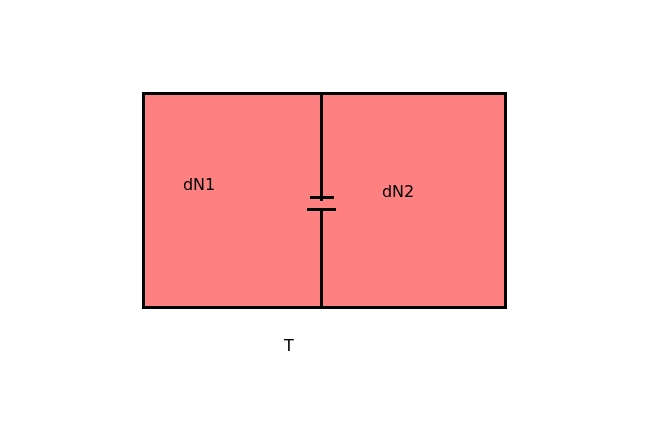
\includegraphics[scale=0.6]{energiaswobodnaczasteczki.jpeg}
			\caption{Energia swobodna a liczba cząstek przy stałej temperaturze}
		\end{figure}
		\begin{equation}
		dN_1 = -dN_2
		\end{equation}
		\begin{equation}
		dF = dF_1 + dF_2 = \frac{\partial F_1}{\partial N_1}dN_1 + 
		\frac{1}{2}\frac{\partial^2 F_1}{\partial N_1^2}(dN_1)^2 +
		\frac{\partial F_2}{\partial N_2}dN_2 + 
		\frac{1}{2}\frac{\partial^2 F_2}{\partial N_2^2}(dN_2)^2
		\end{equation}		
		\begin{equation}
		dF \geqslant 0
		\end{equation}
		\begin{equation}
		dF = \mu_1dN_1 - \mu_2dN_2 \Rightarrow \mu_1 = \mu_2 
		\end{equation}
		Gdyż pierwszy człon rozwinięcia Taylora musi się zerować
		\begin{equation}
		\mu = \mu(T, p, \frac{N}{V}) = \mu(T, p, P)
		\end{equation}
		\begin{equation}
		G = \mu N
		\end{equation}
		\begin{equation}
		\frac{\partial G}{\partial N} = \mu
		\end{equation}
		\textbf{Reguła Gibbsa}
		Reakcje chemiczne: 
		\begin{equation}
		2H_2 + O_2 \rightleftharpoons 2H_2O
		\end{equation}
		Stała postępu reakcji ($ \lambda $ - stała ekstensywna) - liczba wszystkich elementów procesów w skali molekularnej
		\begin{equation}
		dN_{H_2} = -2d\lambda, dN_{O_2} = -d\lambda, dN_{H_2O} = +2d\lambda
		\end{equation}
		\begin{equation}
		dG = dG_{H_2} + dG_{O_2} + dG_{H_2O} =
		 \mu_{H_2}dN_{H_2} + \mu_{O_2}dN_{O_2} + \mu_{H_2O}dN_{H_2O} =
		 (-2\mu_{H_2} - \mu_{O_2} + 2\mu_{H_2o})d\lambda
		\end{equation}
		\begin{equation}
		dG \geqslant 0
		\end{equation}
		jeżeli G jest w stanie równowagi (przyjmuje minimum).\\
		Warunkiem równowagi chemicznej jest:
		\begin{equation}
		-2\mu_{H_2} - \mu_{O_2} + 2\mu_{H_2O} = 0
		\end{equation}
		Potencjał chemiczny zmienia się podczas reakcji. \textbf{R} - liczba reakcji w układzie.
		\begin{equation}
		\lambda^{(k)}, k=1,2,3...,R
		\end{equation}
		\begin{equation}
		\partial N_1 = \sum_{k=1}^{R} v_i^{(k)}d\lambda^{(k)}
		\end{equation}
		$ v_I^{(k)} $ - współczynnik stechiometryczny związku \textit{i} w czasie reakcji \textit{k}.
		\begin{equation}
		dG = Vdp - SdT + \sum_{i=1}^{I}dN_i\mu_i
		\end{equation}
		gdzie \textit{I} to liczba związków chemicznych
		\begin{equation}
		dG = Vdp - SdT + \sum_{i=1}^{I} ( \sum_{k=1}^{R} v_i^{(k)}d\lambda^{(k)} )\mu_i = 
		Vdp - SdT + \sum_{k=1}^{R}d\lambda^{(k)}
		\sum_{i=1}^{I}\mu_i v_i^{(k)} \geqslant 0
		\end{equation}
		Druga suma na końcu 51 jest równa zeru gdy występuje równowaga chemiczna.
		\paragraph{Dla quasi-cząstek, które rozpadają sie bez praw zachowania:}
		\begin{equation}
		\varepsilon_i = \hbar \nu _i, T
		\end{equation}
		Przykłady quasi-cząstek: foton, fonon(kwant pola sprężystości), magnenon(kwant uporządkowania magnetycznego).
		\begin{figure}[ht]
			\label{fig:fig1}
			\centering
			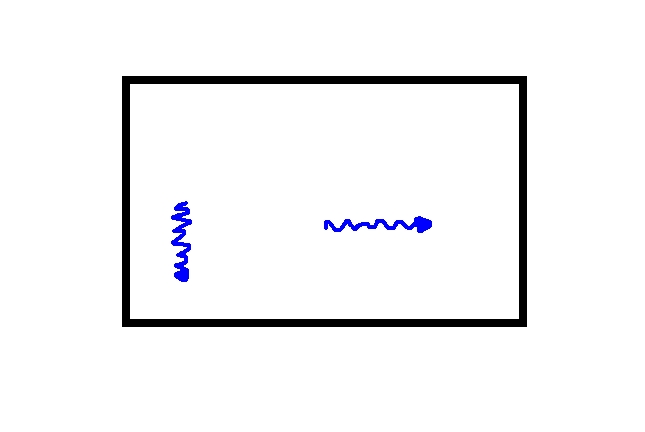
\includegraphics[scale=0.6]{quasiczastki.jpeg}
			\caption{Quasi-cząstki}
		\end{figure}
		\begin{equation}
		0 \leqslant dG = \sum_{i}^{}dN_i\mu_i
		\end{equation}
		Jeżeli $ dN_i $ jest dowolne, to $ \mu_i = 0 $
		\begin{equation}
		\begin{Bmatrix}
			G(T, p, N) = \mu N \\
			\frac{\partial G}{\partial N} = \mu \\
			G = G_{min}
		\end{Bmatrix}
		\Rightarrow \frac{\partial^2 G}{\partial N^2} = 
		\frac{\partial \mu}{\partial N} \geqslant 0
		\end{equation}
		\paragraph{Termodynamika przejść fazowych}
		\begin{figure}[ht]
			\label{fig:fig1}
			\centering
			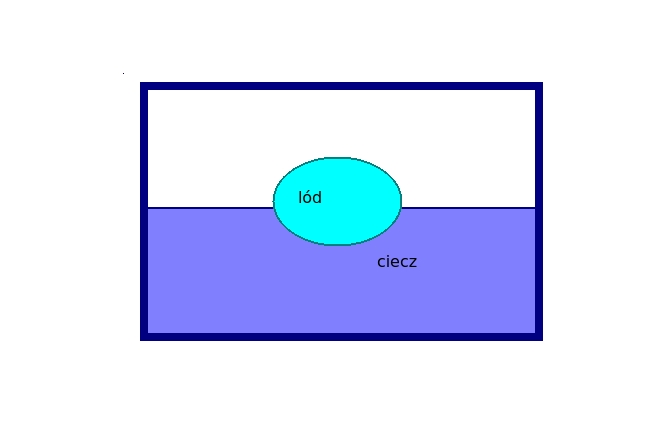
\includegraphics[scale=0.6]{termodynamikaprzejsc.jpeg}
			\caption{Termodynamika przejść fazowych}
		\end{figure}
		\begin{equation}
		\mu_{lod} = \mu_{ciecz}
		\end{equation}
		P różnych faz w równowadze. $ P \geqslant 1 $\\
		B różnych związków $ (H_2O, NaCl) $\\
		$ \mu_a^{(b)} $ - potencjał chemiczny związku \textit{a} w fazie \textit{b}
		\begin{equation}
			\begin{rcases}
				\mu_1^{(1)}=\mu_1^{(2)}=\mu_1^{(3)} = ... =\mu_1^{(P)} \\
				\mu_2^{(1)}=\mu_2^{(2)}=\mu_2^{(3)} = ... =\mu_2^{(P)} \\
				\vdots \\
				\mu_B^{(1)}=\mu_B^{(2)}=\mu_B^{(3)} = ... =\mu_B^{(P)} \\
			\end{rcases}
		\end{equation}
		$ (P-1) \dot B $ równań - więzy na potencjały chemiczne	
		Zmienne swobodne(argumenty $ \mu_a^{(b)} = \mu_a^{(b)}(T, p, p_a^{(b)}, p_{a'}^{(b)}, p_{a''}^{(b)}, ...)$) \\
		$ C_a^{(b)} $ - koncentracja związku \textit{a} w fazie \textit{b} \\
		\begin{equation}
		\sum_{a}^{}C_a^{(b)} = 1
		\end{equation}
		\begin{equation}
		Z = 2 + (B -1) \cdot P
		\end{equation}
		Zmienne swobodne
		\begin{equation}
		f = 2 + (B-1)P - (P-1)B = 2 + B - P
		\end{equation}		
		\textbf{Reguła faz Gibbsa}
		\begin{equation}
		f = 2 + B - P - R
		\end{equation}
		dla R reakcji chemicznych. \\
		\paragraph{Klasyfikacja przejść fazowych:}
		Przejście fazowe jest n-tego rzędu jeśli w procesie przejścia fazowego wszystkie pochodne potencjału chemicznego G rzędu n-1 są ciągłe, a przynajmniej jedna pochodna rzędu n jest nieciągła.
	\section{Wykład 6} 
		\begin{equation}
			dG = -SdT + Vdp + \mu dN
		\end{equation}
		Jeżeli $ (\frac{\partial G}{\partial T})_{p,N}$ jest nieciagła to $ S $ też jest nieciągłe. Entropia kryształu jest mniejsza (skokowo) niż entropia cieczy.
		\begin{equation}
		S_{cieczy} = S_{kryształu} + \Delta S = \frac{Q_{topnienia}}{T}
		\end{equation}
		Jeżeli ciepło przemiany fazowej jest różne od zera to przejście fazowe jest \textbf{pierwszego rzędu}. \\
		Jeżeli $ (\frac{\partial G}{\partial p})_{T,N} $ jest nieciągła to $ V $ również jest nieciągłe.\\
		Objętość kryształu jest mniejsza (skokowo) niż objętość cieczy.
		\begin{equation}
		V_{cieczy} = V_{kryształu} + \Delta V
		\end{equation}
		Jeżeli różnica objętości podczas przemiany fazowej jest różna od zera to przejście fazowe jest \textbf{pierwszego rzędu}.
		Jeżeli $ (\frac{\partial ^ 2 G}{\partial S ^ 2})_{p,N} $ jest nieciągła to $ \frac{\partial S}{\partial T} $ też jest nieciągła.
		\begin{equation}
		dS = \frac{dQ}{T} \Rightarrow \frac{dS}{dT} = \frac{\frac{dQ}{dT}}{T} = \frac{C_p}{T}
		\end{equation}
		Jeżeli $ C_p $ jest różne dla przejść fazowych, to przejście jest to przejście fazowe \textbf{drugiego rzędu}.
		\begin{figure}[ht]
			\label{fig:fig1}
			\centering
			\
			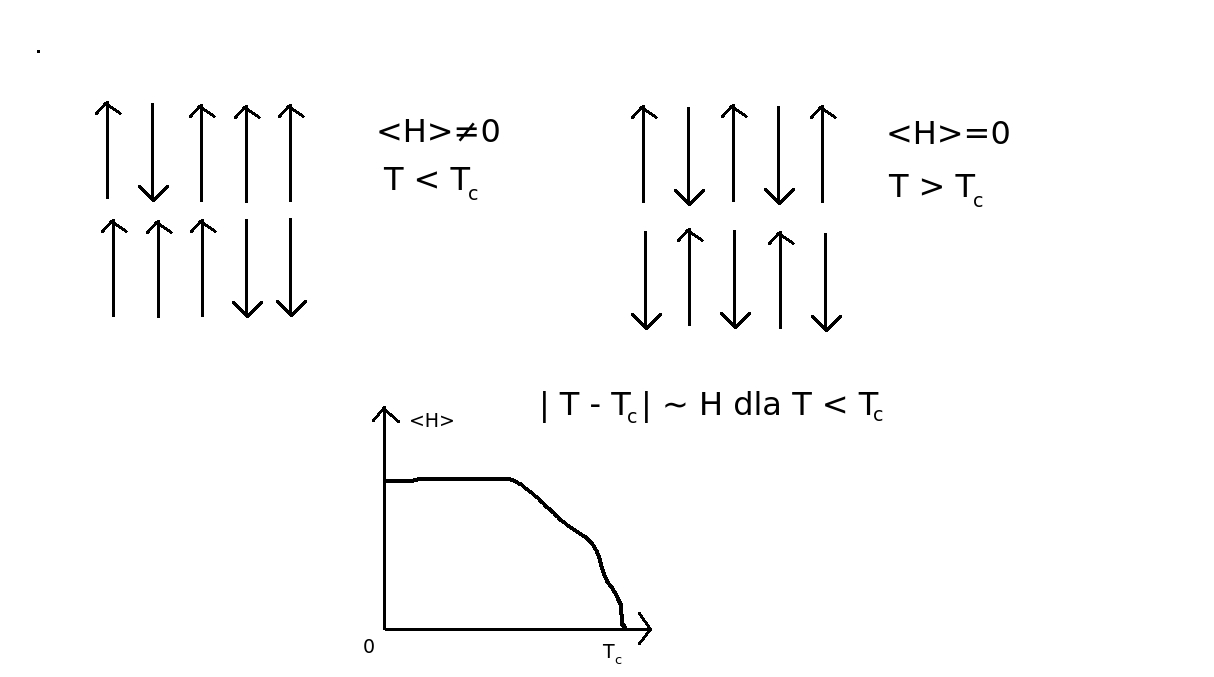
\includegraphics[scale=0.45]{przejsciafazowe.jpeg}
			\caption{Przykład dla przejść fazowych - ferromagnetyk}
		\end{figure}
		\subsection*{III zasada termodynamiki} 
		\begin{equation}
		 S(T \rightarrow 0K) \approx 0  
		\end{equation}
		dokładniej: $ S \approx k_B ln(I)$ i $ I $ jest bardzo małe \\
		\begin{equation}
		S = k_Bln(\Omega)
		\end{equation}  $ \Omega $ - liczba możliwych mikrostanów.
		Gdy $ T \rightarrow 0K$, to $ <U> \rightarrow <U_min> $ (minimum globalne). Krotność degeneracji $ <U_{min}> $ odpowiada kilku stanom układu.
		\paragraph{} Z III zasady termodynamiki wynika ze temperatura $ 0K $ nie może zostać osiągnięta za pomocą skończonej liczby cyklów termodynamicznych. Ponadto: 
		\begin{equation}
		C_p,C_v \xrightarrow{T_k \rightarrow 0K} 0
		\end{equation}
		\paragraph{Prawo Clausius'a-Clapeyron'a (dla przejść fazowych pierwszego rodzaju)}
		\begin{figure}[ht]
			\label{fig:fig1}
			\centering
			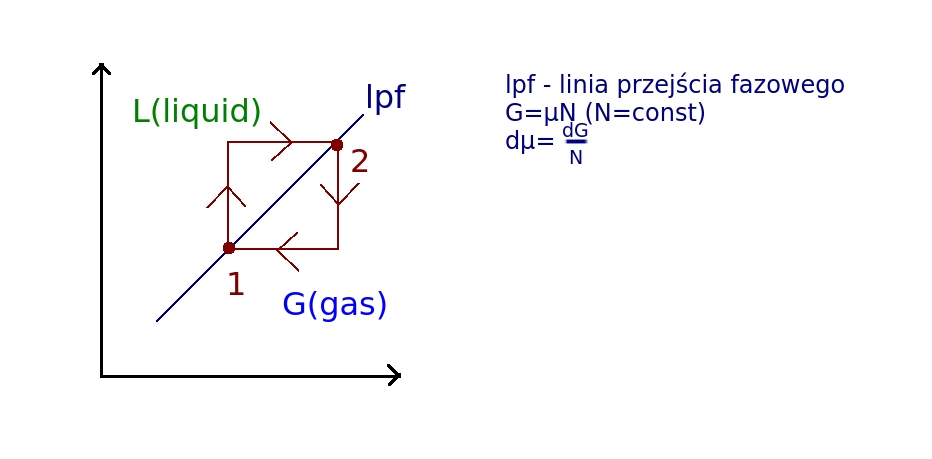
\includegraphics[scale=0.5]{clausius.jpeg}
			\caption{Prawo Clausiusa - Clapeyrona}
		\end{figure}
		\begin{equation}
		d\mu = \frac{-SdT+Vdp}{N}
		\end{equation}
		\begin{equation}
		\mu_L(T,p) = \mu_G(T,p)
		\end{equation}
		\begin{equation}
		d\mu_L = d\mu
		\end{equation}
		\begin{equation}
		-S_LdT + V_Ldp = -S_GdT + V_Gdp
		\end{equation}
		\begin{equation}
		\underbrace{(S_G - S_L)dT}_{\frac{Q_p}{T}} = \underbrace{(V_G - V_L)dp}_{\Delta V} 
		\end{equation}
		\begin{equation}
		\frac{Q_p}{T}dT = \Delta Vdp \Rightarrow (\frac{dp}{dT})_{cpf} = 
		\frac{Q_p}{\Delta VT} \text{  lpf.}
		\end{equation}
		\paragraph{FIZYKA STATYSTYCZNA}
		Przestrzeń fazowa $ \Omega $
		\begin{equation}
		\Omega = \{ \lceil \vec{r_1}, \vec{p_1} ,..., \vec{r_N}, \vec{p_N} \rceil\}
		\end{equation}
		Zbiór wektorów 6N - wymiarowych.
		\begin{equation}
		\uparrow \uparrow \uparrow \downarrow \downarrow \uparrow \downarrow \downarrow 
		\end{equation}
		Momenty magnetyczne $ \Omega = \underbrace{\{ \lceil 1,1,1,-1-1,1,-1,-1 \rceil\}}_{N} $, $ d\Gamma $ - unormowane elementy przestrzeni fazowej.
		\begin{equation}
		d\Gamma = \frac{d^3r_1d^3p_1...d^3r_Nd^3p_N}
		{N!\cdot \hbar^{3N}}
		\end{equation}
		Wielkości makroskopowe są średnimi po czasie (trajektorii) wielkości makroskopowych.
		\begin{equation}
		<f(t)>_t = <f>_p
		\end{equation}
		\begin{figure}[ht]
			\label{fig:fig1}
			\centering
			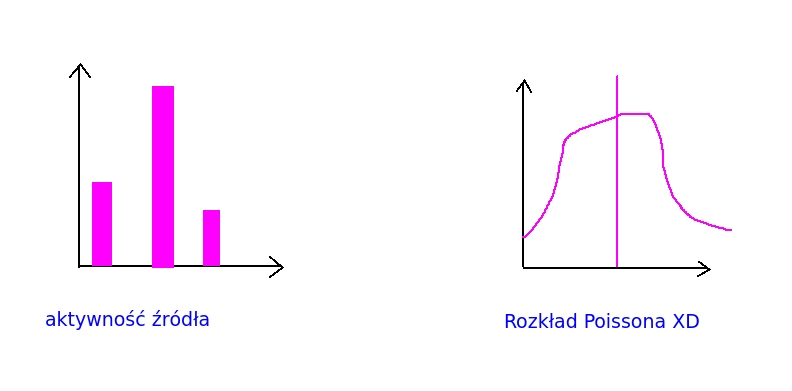
\includegraphics[scale=0.5]{statystyczna.jpeg}
			\caption{Prawo Clausiusa - Clapeyrona}
		\end{figure}
	\section{Wykład 7}
		\subsection*{3 zespoły statystyczne}
		\paragraph{Zespół statystyczny} to zbiór kopii tego samego układu w różnych mikrostanach, a tym samym makrostanem.
		\paragraph{}Wyróżniamy 3 zespoły statystyczne:
		\begin{itemize}
			\item Układ izolowany: zespół mikrokanoniczny 
			\begin{equation}
			N,E,V=const
			\end{equation}
			\item Układ zamknięty: zespół kanoniczny
			\begin{equation}
			N,V = const
			\end{equation}
			\item Układ otwarty: zespół makrokanoniczny
		\end{itemize}
		\begin{equation}
		\text{zespół statystyczny} \longleftrightarrow \text{statystyczny rozkład prawdopodobieństwa}
		\end{equation}
		\paragraph{Dla zespołu mikrokanonicznego:}
		\begin{equation}
		P(\Omega) = \frac{1}{\Delta \Gamma}
		\end{equation}
		Gdzie $ \Omega $ to przestrzeń fazowa opisująca mikrostany a $ \Delta \Gamma $ to objętość dozwolonej przestrzeni fazowejht
		\begin{equation}
		S = k_Bln(\Delta \Gamma)
		\end{equation}
		\paragraph{Przykład: oscylator harmoniczny}
		\begin{figure}[ht]
			\label{fig:fig1}
			\centering
			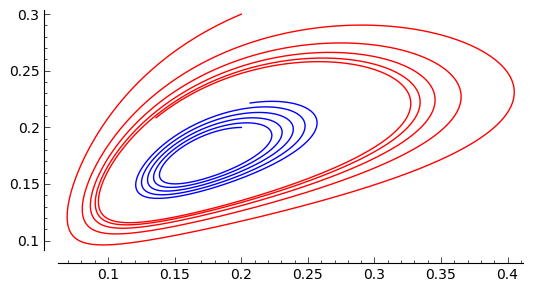
\includegraphics[scale=0.5]{przestrzenfazowa.png}
			\caption{Przestrzeń fazowa oscylatora harmonicznego}
		\end{figure}
		\begin{equation}
		H = \frac{p^2}{2m} + \frac{m\omega^2x^2}{2}
		\end{equation}
		\begin{equation}
		x=x_0sin(\omega t)
		\end{equation}
		\begin{equation}
		p=p_0cos(\omega t)
		\end{equation}
		$ \Delta \Gamma $ to pole tego kształtu.
		\begin{figure}[ht]
			\label{fig:fig1}
			\centering
			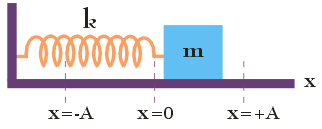
\includegraphics[scale=0.5]{oscylator.png}
			\caption{Oscylator harmoniczny}
		\end{figure}
		\begin{equation}
		\sum_{elipsy}^{} = \pi x_0p_0
		\end{equation}		
		
		\begin{equation}
			E = \frac{kx_0^2}{2} = \frac{m\omega^2x^2}{2} \pm \frac{p_0^2}{2m}
		\end{equation}
		\begin{equation}
		\sum_{elipsy}^{} = 
		\pi \frac{1}{\omega}\sqrt{\frac{2E}{m}}\cdot \sqrt{2mE} = 
		\frac{2\pi}{\omega}E
		\end{equation}
		\begin{equation}
		\Delta \Gamma = \Sigma_2 - \Sigma_1 = \frac{2\pi}{\omega}\Delta E
		\end{equation}
		\begin{equation}
		\Delta \tilde{\Gamma} = \frac{\Delta\Gamma}{h}
		\end{equation}
		Znormalizowana objętość przestrzeni fazowej
		\paragraph{}
		\begin{equation}
		X=X(x,p)
		\end{equation}
		gdzie X jest obserwablą
		\begin{equation}
		<X>_t = \frac{1}{T\Delta E} \int_{E}^{E + \Delta E}\int_{0}^{T}X(t,E)dtdE
		\end{equation}
		gdzie
		\begin{equation}
		x = x(t,E),
		p = p(t,E)
		\end{equation}
		\begin{equation}
		x = \sqrt{\frac{2E}{m\omega^2}}sin(\omega t)
		\end{equation}
		\begin{equation}
		p = \sqrt{2Em} cos(\omega t)
		\end{equation}
		Chcemy wymienić zmienne $ (E,t) \longrightarrow (x,p)$
		\begin{equation}
		y=
		\begin{vmatrix}
		\frac{\partial x}{\partial t} && \frac{\partial x}{\partial E} \\
		\frac{\partial p}{\partial t} && \frac{\partial p}{\partial E}
		\end{vmatrix}
		=
		\begin{vmatrix}
		\sqrt{\frac{2E}{m\omega ^2}}\omega cos(\omega t) && \sqrt{\frac{1}{2Em\omega^2}}sin(\omega t) \\
		-\sqrt{2Em}\omega sin(\omega t) &&\sqrt{\frac{m}{2E}}cos(\omega t)
		\end{vmatrix}
		=1
		\end{equation}
		\begin{equation}
		<X>_t = \frac{\omega}{2 \pi} \cdot \frac{1}{\Delta E} \int\int X(x,p) \cdot \underbrace{1}_{Jakobian} \cdot dxdp
		\end{equation}
		Całkujemy po "obwarzanku".
		\begin{equation}
		\Delta \Gamma = \frac{2\pi}{\omega h}\Delta E
		\end{equation}
		Co wynika z poprzednich rozważań.
		\begin{equation}
		<X>_t = \frac{1}{h\Delta \Gamma}\int\int X(x,p)dxdp = 
				\frac{1}{\Delta \Gamma}\int\int X(x,p)\frac{dxdp}{h}
		\end{equation}
		\begin{equation}
		P(x,p) = \frac{1}{\Delta \Gamma} = P(\Omega)
		\end{equation}
		\begin{equation}
		S = k_Bln(\Delta \Gamma) = -k_Bln(P_0)
		\end{equation}
		\begin{figure}[ht]
			\label{fig:fig1}
			\centering
			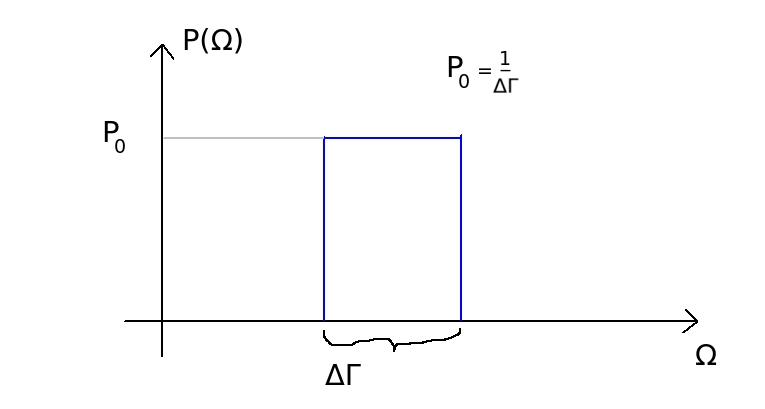
\includegraphics[scale=0.5]{przestrzenoscylator.jpeg}
			\caption{Przestrzeń fazowa}
		\end{figure}
		\paragraph{Zespół kanoniczny}
		\begin{figure}[ht]
			\label{fig:fig1}
			\centering
			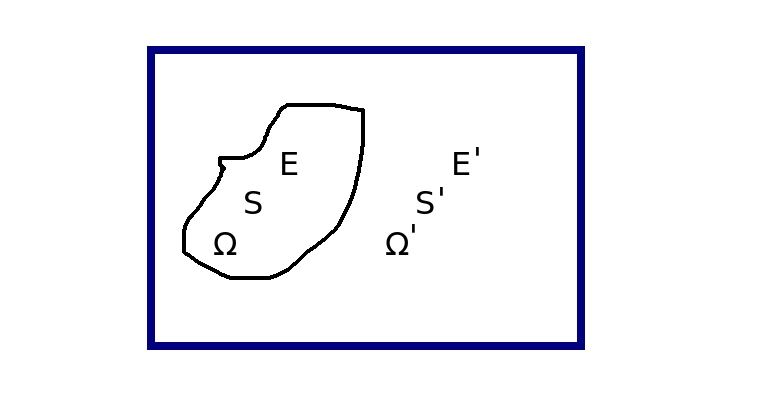
\includegraphics[scale=0.5]{kanoniczny.jpeg}
			\caption{Zespół kanoniczny}
		\end{figure}
		\begin{equation}
		\text{układ} + \text{termostat} = \text{nadukład izolowany}
		\end{equation}
		\begin{equation}
		E << E'
		\end{equation}
		\begin{equation}
			\begin{array}{cc}
			 E + E' = E_t \\
			 S + S' = S_t \\
			 \text{t - total}
			\end{array}
		\end{equation}
		\begin{equation}
		P(\Omega, \Omega ') = \frac{1}{\Delta \Gamma_t}
		\end{equation}
		\begin{equation}
		\begin{array}{cc}
		P(\Omega) ~ \Delta \Gamma'(E') = exp(\frac{S'}{k_B}) = \\
		= exp(\frac{S'(E')}{k_B}) = exp(\frac{S'(E_t - E)}{k_B}) = 
		\Big \langle S'(E_t) + \frac{\partial S'}{\partial E'} dE \Big \rangle = \\
		= exp \lceil \frac{1}{k_B}(S'(E_t) - \frac{E}{T})\rceil = 
		\frac{1}{2} exp\lceil \frac{-E}{k_BT} \rceil
	
		\end{array}
		\end{equation}
	\section{Wykład 8}
		\begin{equation}
		P(\Omega) = \frac{1}{Z}e^{-\beta E(\Omega} \text{ i } \beta = \frac{1}{k_BT}
		\end{equation}
		Gdzie Z to suma stanów (suma statystyczna). Aby obliczyć $ z $ należy:
		\begin{equation}
		\int e^{-\beta E}d\Omega = z \text{ lub } \sum_{\Omega}^{} e^{-\beta E} = z
		\end{equation}
		\begin{equation}
		z = z(\Omega)
		\end{equation}
		\begin{equation}
		\begin{array}{cc}
		U = <E> = \sum_{\Omega}^{}E(\Omega)P(\Omega) = \frac{1}{Z}\sum_{\Omega}^{}E(\Omega)e^{-\beta E(\Omega)} =\\ \\
		=\frac{-1}{z}\frac{\partial }{\partial \beta} \underbrace{\sum_{\Omega}^{}e^{-\beta E(\Omega)}}_{z} = -\frac{1}{z} \cdot z' = -\frac{\partial}{\partial \beta} \lceil ln(z) \rceil
		\end{array}{}
		\end{equation}
		\begin{equation}
		S = k_B ln(\Delta \Gamma) = -k_Bln(P_0)
		\end{equation}
		gdzie $ P_0 = \frac{1}{\Delta \Gamma} $ - \textbf{rozkład mikrokanoniczny}
		\begin{equation}
		S = -k_B \int P(\Omega) ln\lceil P(\Omega) \rceil d\Omega
		\end{equation}
		\paragraph{Postulat:} obliczone S w (111) sprawdza się dla każdego rozkładu.
		\begin{equation}
		S = -k_B<ln\lceil P(\Omega) \rceil>
		\end{equation}
		\begin{equation}
		S = -k_B<-ln(z) - \beta E(\beta)> = k_Bln(z) + \frac{k_B}{k_BT}<E(\Omega)> = k_Bln(z) + \frac{U}{T}
		\end{equation}
		\begin{equation}
		F = U - TS = U - T(k_Bln(Z) + \frac{U}{T}) = - k_BTln(z) \Rightarrow z = e^{-\beta F}
		\end{equation}
		Zespół kanoniczny jest w przybliżeniu zespołem mikrokanonicznym.
		\begin{equation}
		\frac{\partial E}{<E>} \xrightarrow[N \Rightarrow \infty]{} 0 \text{ i } \frac{\partial E}{<E>} ~ \frac{1}{\sqrt{N}} \text{ i } \delta E \text{ to fluktuacje energii}
		\end{equation}
		\paragraph{Dowód:}
		\begin{equation}
		\begin{array}{cc}
		\sigma^2_E = \sigma^2 = <(E-U)^2> = <E^2> - <E>^2 = \langle <E> = -\frac{\partial}{\partial \beta} ln(z) \rangle = \\ \\
		= \sum_{\Omega}^{}E^2(\Omega) \cdot \frac{1}{z}e^{-\beta E} - 
		\lceil \frac{\partial}{\partial \beta} ln(z)\rceil^2 = 
		\frac{1}{z} \frac{\partial ^2}{\partial \beta^2} \sum_{\Omega}^{} e^{-\beta E} - 
		\lceil \frac{\partial}{\partial \beta}ln(z)\rceil^2 = \\ \\
		= \frac{z''}{z} - (\frac{z'}{z})^2 = \frac{zz'' - (z')^2}{z^2} = (\frac{z'}{z})' = 
		-\frac{\partial}{\partial \beta}U
		\end{array}
		\end{equation}
		\begin{equation}
		\sigma ^2 = - (\frac{\partial U}{\partial T})_V \cdot \frac{\partial T}{\partial \beta} = C_V \cdot k_BT^2 = 
		(k_BT) \cdot Tc_V \sim N
		\end{equation}
		\begin{equation}
		\sigma^2 \sim N \Rightarrow \sigma \sim \sqrt{N}
		\end{equation}
		\begin{equation}
		\frac{\sigma}{E} \sim \frac{1}{\sqrt{N}} \xrightarrow[N \rightarrow \infty]{} 0 \text{ \textbf{cnd.} }
		\end{equation}
		\paragraph{Jeżeli mamy układ nieoddziałujący to:}
		\begin{equation}
		E = E_1 + E_2 + ... + E_N
		\end{equation}
		\begin{equation}
		e^{-\beta E} = e^{-\beta E_1} \cdot e^{-\beta E_2} \cdot ... \cdot e^{-\beta E_N}
		\end{equation}
		\begin{equation}
		z = \sum_{\Omega_1}^{}\sum_{\Omega_2}^{}...\sum_{\Omega_N}^{}e^{-\beta E} = 
		Z_1\cdot Z_2 \cdot ... Z_N
		\end{equation}
		Powyżej: multiplikatywność sumy statystycznej.
		\paragraph{Wielki rozkład kanoniczny (makrokanoniczny)}
		\begin{figure}[ht]
			\label{fig:fig1}
			\centering
			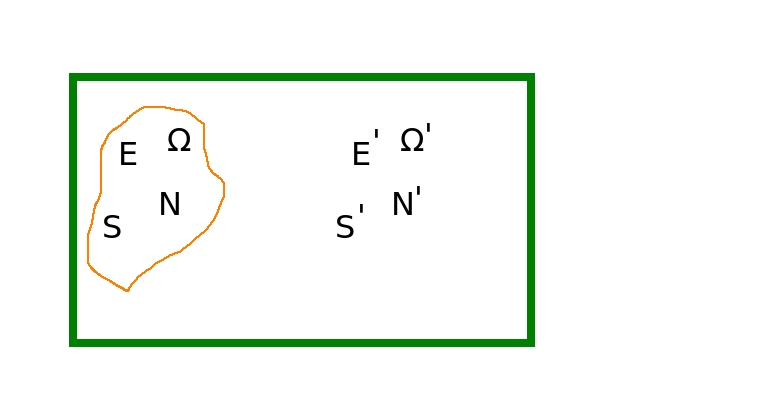
\includegraphics[scale=0.5]{wielkikanoniczny.jpeg}
			\caption{Wielki rozkład kanoniczny}
		\end{figure}
		\begin{equation}
		N + N' = N_t \text{ , } S + S' = S_t \text{ , } E + E' = E_t
		\end{equation}
		\begin{equation}
		\begin{array}{cc}
			P(\Omega, N) \sim \Delta \Gamma' = exp\lceil \frac{S'}{k_B} \rceil = 
			exp\lceil \frac{S'(E',N')}{k_B} \rceil= \\ \\
			 = exp\lceil {S'(E',N')}\frac{1}{k_B} {S'(E_t - E,N_t - N)} \rceil= \\ \\ 
			 = exp\lceil \frac{1}{k_B}(S'(E_t, N_t) + (-E)\frac{\partial S'}{\partial t'} + 
			 (-N)\frac{\partial S'}{\partial N'} \rceil = \\ \\
			 = \langle dS = \frac{dU - \mu dN}{T} \rangle = 
			 exp \lceil C + \frac{1}{k_B} (\frac{N\mu}{T} - \frac{E}{T})
		\end{array}
		\end{equation}
		\begin{equation}
		P(\Omega, N) = \frac{1}{\dot{z}} e^{-\beta (E - \mu N)}
		\end{equation}
		Gdzie $ \dot{z} $ to wielka suma statystyczna.
		\begin{equation}
		\dot{z} = \sum_{Z}^{}\sum_{\Omega_N}^{}e^{-\beta (E - \mu N)}
		\end{equation}
		\begin{equation}
		\dot{z}_{12} = \dot{z}_1 \cdot \dot{z}_2
		\end{equation}
		\begin{equation}
		\begin{array}{cc}
		<N> = \sum_{Z}^{}\sum_{\Omega_N}P(\Omega_N, N) \cdot N = \\ \\
		 = \sum_{Z}^{}\sum_{\Omega_N}\frac{1}{\dot{z}}e^{-\beta (E - \mu N)} = \\ \\
		 \frac{1}{\dot{z}} \sum_{Z}^{}\sum_{\Omega_N} \frac{1}{\beta}\frac{\partial}{\partial \mu} 
		 e^{-\beta (E_N - \mu N)} = k_BT\frac{\partial}{\partial \mu}\lceil ln(\dot{z})\rceil
		\end{array}
		\end{equation}
	\section{Wykład 9}
		Dla wielkiego rozkładu kanonicznego:
		\begin{equation}
		S = -k_B<ln(P)>
		\end{equation}
		\begin{equation}
		P(\Omega_N, N) = \frac{1}{\dot{Z}}e^{-\beta(E(\Omega) - \mu N)}
		\end{equation}
		\begin{equation}
		\begin{array}{cc}
			S = -k_B \lceil - ln(\dot{z}) - <\beta(E - \mu N)> \rceil = 
			k_Bln(\dot{z}) + \frac{1}{T}(<E> - \mu<N>) = \\ \\
			k_Bln(\dot{z}) + \frac{U}{T} - \frac{\mu}{T}<N>
		\end{array}
		\end{equation}
		\begin{equation}
		F = U - TS = U - T(k_Bln(\dot{z}) + \frac{U}{T} - \frac{\mu}{T}<N>) = -k_BTln(\dot{z}) + \mu <N>
		\end{equation}
		\begin{equation}
		G = \mu <N>
		\end{equation}
		(134) wynika z definicji.
		\begin{equation}
		F = G - k_BTln(\dot{z})
		\end{equation}
		(135) wynika z przyrównania (134)
		\begin{equation}
		G = F + pV
		\end{equation}
		(136 z definicji)
		\begin{equation}
		F = F + pV - k_Bln(\dot{z})
		\end{equation}
		\begin{equation}
		pV = k_BTln(\dot{z})
		\end{equation}
		(138) to \textbf{równianie stanu}.
		\paragraph{Przykład: układ oscylatorów}
		\begin{equation}
		H_i = \frac{kx_i^2}{2} + \frac{p_i^2}{2m}
		\end{equation}
		\begin{equation}
		H = \sum_{i=1}^{N}H_i
		\end{equation}
		Zakładamy że $ k $ i $ m $ są takie same.
		\begin{equation}
		z_N = (z_1)^N
		\end{equation}
		\begin{equation}
		\begin{array}{cc}
			z_1 = \int_{- \infty}^{\infty} \int_{- \infty}^{\infty} 
			e^{-\beta(\frac{kx^2}{2} + \frac{p^2}{2m})}dxdp = \\ \\
			= \int_{- \infty}^{\infty}exp\lceil -\beta \cdot \frac{kx^2}{2}dx \rceil \cdot
			\int_{- \infty}^{\infty}exp\lceil -\beta \cdot  \frac{p^2}{2m}dp \rceil = \\ \\
			\langle \int_{- \infty}^{\infty} e^{-ax^2}dx = \sqrt{\frac{\pi}{a}} \rangle =
			\sqrt{\frac{\pi}{\frac{k\beta}{2}}} \cdot \sqrt{\frac{\pi}{\frac{\beta}{2m}}} = 
			2\pi k_B T\sqrt{\frac{m}{k}}
		\end{array}
		\end{equation}
		\begin{equation}
		Z_N = (2\pi k_B T)^N(\frac{m}{k})^{\frac{N}{2}} = A\beta^{-N} \text{ , A = const} 
		\end{equation}
		\begin{equation}
		U = -\frac{\partial}{\partial \beta}ln(z) = -\frac{\partial}{\partial \beta} 
		\lceil ln(A) - Nln(\beta) \rceil = \frac{N}{\beta} = k_BT \cdot N 
		\end{equation}
		Dla układu trójwymiarowego $ U = k_BT \cdot 3N $ ciepło właściwe: 
		\begin{equation}
		C_V = (\frac{dU}{dT})_V = 3N\cdot k_B
		\end{equation}		
					
		
		
		
		
		
		
		
		
		
\end{document}
